% Class:
\documentclass{report}

% Fonts:
\usepackage[T1]{fontenc}
\usepackage{lmodern}
% Links:
\usepackage{hyperref}

% Maths:
\usepackage{amsmath}
\usepackage{amssymb}
\usepackage{mathrsfs,amsmath}
\newcommand{\e}[1]{\times 10^{#1}}
\usepackage{siunitx}

% Figures:
\usepackage{graphicx}
\usepackage{caption}
\usepackage{subcaption}
\graphicspath{ {./} }
\usepackage{float}

% Footnotes:
\usepackage[symbol]{footmisc}
\renewcommand{\thefootnote}{\fnsymbol{footnote}}

% Others:
\usepackage{pdfpages}
%\usepackage[backend=bibtex]{biblatex}
\usepackage{textcomp}
\usepackage{pdflscape}

% Title:
\title{
	Sound-source Localisation using a Microphone-array for NUbots\\
	Interim Report
}
\author{Clayton Carlon, C3327986}
\date{\today}

% Document:
\begin{document}

\maketitle

\chapter{Introduction}

Locating a source of sound is a long sought after ability in technology, especially in the study and development of robotics which seeks to emulate and compete with human senses. The main aspiration for this project is to develop an array of microphones along with an accompanying computation, preferably embedded, to locate a source of sound using signal-processing techniques. In the end, this system will be used on the football-playing robots in the NUbots team, the university's on-campus robotics team.

\section{Background}

NUbots is a multidisciplinary team under the University of Newcastle's robotics research group and has competed since 2002 in RoboCup, an international competition where humanoid robots play association-football\footnote{otherwise known as football or soccer}. The team is multidisciplinary and is made up of both undergraduate and postgraduate students in computer science and engineering. At this time, the robots on the team are modified versions of the igus\textregistered\ Humanoid Open Platform; this modified platform is called the NUgus hardware platform and competes in the kid-size league.

The remit of the team is broad and is not only competing in the RoboCup. Although it strives to win RoboCup, the team also does research more generally in areas related to robotics, such as computer-vision, robotic locomotion and control, etc. Therefore, the project does not necessarily have to be tied to the said competition. Furthermore, this project, as it evolves, does not necessarily have to be used in the application of NUbots nor robotics more generally although the original idea came from NUbots. Sound-source-localisation is a broad area of study, and the final prototype can just as easily be employed in other applications, such as a video-conference-system, drones, etc.

\section{Scope}

Ideally, the project shall yield a working prototype fitted on one of the NUgus robots. At this time, since the project is more intended as a proof-of-concept, its goals are thus somewhat open-ended. However, such basic goals are that it should at the very least:
\begin{itemize}
	\item estimate the three-dimensional direction, i.e. the azimuth and the elevation,
	\item locate a reasonably distinct sound in a moderate environment, e.g. a whistle, a lone voice, a loud thud,
	\item and handle the noise from the motors of the robot which will nearby.
\end{itemize}
Further goals are that it can:
\begin{itemize}
	\item estimate the distance along with direction, essentially locate the source's full coordinates in three-dimensions,
	\item track the location over time using e.g. a Kalman filter,
	\item locate multiple simultaneous sources, as long as they have relatively distinct locations,
	\item spatially filter the localised sound,
	\item and work well enough in noisy and reverberant environments, e.g. in a hall full of people.
\end{itemize}

% accuracy 

Although sound-source-localisation will be helpful in a scenario of football-playing robots, the final system does not have to directly help the robot's performance in a match. The ability for a robot to interact with humans is a broad and well sought after goal. Even a basic demonstration of the robot turning its head towards a human speaker can help the team's outreach and marketing in exhibition-shows, publicity-events, etc. Not only will this help sponsors and thus funding for the team, but even the basic proof of concept also contributes further to the team's research in and remit of robotics 

\chapter{Literature-Review}

Since sound-source-localisation is a much widely researched problem, in e.g. robotics, drones, video-conferencing, the military, submarines, hearing aids, etc., the review of the literature can be quite broad. To narrow the search, and to also find examples that are most relevant to this project, especially for computation and dimensions, this review has mostly considered literature with a robotics context, rather than large-scale military outdoor application for example. Indeed, sound-source-localisation for drones shares a good deal with that for robotics, e.g. the influence of motors, but one important difference is the fact that applications for drones are mostly outdoors rather than indoors where the reverberation is an important factor.

To further help narrow the scope of the search, most methods considered are ones that use an array of at least two microphones and use some kind of signal-processing. Other families of methods exist such as binaural approaches with two microphones and head-models \cite{argentieri_survey_2015} and those that use machine-learning, such as convolutional neural networks \cite{sakavicius_multiple_2022}. It is not necessarily that these other approaches will be ignored outright but rather that the scope of the literature-review as well as the project as a whole will be kept relevant in order to ease the search.

\section{Methods}

\subsection{Overview}

There are already a few reviews of the literature, each going through a number of existing and studied methods for sound-source-localisation. A survey \cite{argentieri_survey_2015} attempted to give a state of the art of sound-localisation in robotics. It dealt with two main areas, namely binaural approaches and array-based approaches. Since an array of microphones will be used in this project, the latter area is most relevant. All the approaches of which that the survey explored were listed as such:
\begin{itemize}
	\item MUSIC,
	\item TDOA, and
	\item beam-forming.
\end{itemize}

Another review \cite{rascon_localization_2017} also classified methodologies as:
\begin{itemize}
	\item one-dimensional single direction-of-arrival estimation,
	\item two-dimensional single direction-of-arrival estimation,
	\item multiple direction-of-arrival estimations, and
	\item distance-estimation.
\end{itemize}
Here, the review talks about correlation as a way to estimate a single direction of arrival and about beam-forming and MUSIC as a way to estimate multiple directions. It also discusses the potential use of correlation for multiple sources given that other sources are represented as secondary peaks. 

To estimate the distance, the review proposes a number of ways, some of which are:
\begin{itemize}
	\item the intersection of hyperbolic curves from multiple estimated TDOA,
	\item triangulation of multiple DOA at different positions of the robot using its mobility,
	\item triangulation of multiple DOA from different sub-arrays,
\end{itemize}

One important distinction about the geometry is the far field and the near field. Many methods approximate their algorithm and computation by assuming that the source is in the far field where the distance between the source and the array is comparably longer than the array's width. This is such that the sound-waves may be assumed to be planar at the array and such that the direct lines between the source and each microphone may be assumed to be parallel. Some methods, especially those of beam-forming, can estimate distance but only in the near field where the distance between the source and the array is comparable to the array's width. However, since the microphone-arrays in robotic applications are generally small, only the far field is an acceptable assumption. This may especially be the case for NUbots where candidate space for an array on the existing NUgus is sparse and a smaller array may have to be chosen.

\subsection{Time-Difference of Arrival}

A simple yet proven way to estimate the DOA of a sound-source using a microphone-array is to calculate the difference in time \cite{argentieri_survey_2015}. Commonly, the TDOA of two microphones is often found by the cross-correlation of two signals, the highest peak of which corresponds to the estimated TDOA. 
\begin{equation}
R_{ij}(\tau) = \sum_{n=0}^{N-1} x_i[n]x_j[n-\tau]
\end{equation}
where $x_i$ and $x_j$ are the two signals, from two microphones for example. Cross-correlation is useful in particular because it has an equivalent calculation in the frequency-domain:
\begin{equation}
R_{ij}(\tau) = \mathfrak{F}^{-1} \left( X_i[k]X_j[k]^* \right)
\end{equation}
where $X_i[k]$ and $X_j[k]$ are the Fourier transforms of $x_i$ and $x_j$ respectively. Unlike the original calculation which relies on addition and has a complexity of $O(N^2)$, this frequency-domain equivalent relies on multiplication, can be made more efficient by FFT, and has a complexity of $O\left(N\ln(N)\right)$ \cite{valin_robust_2003}.

An advanced form of this TDOA estimation is the generalised cross-correlation (GCC):
\begin{equation}
R^{(w)}_{ij}(\tau) = \mathfrak{F}^{-1} \left( \psi[k]X_i[k]X_j[k]^* \right)
\end{equation}
where $\psi[k]$ is the spectral weighting \cite{argentieri_survey_2015}, \cite{rascon_localization_2017}. A common weighting is the phase-transform (GCC-PHAT):
\begin{equation}
\psi[k] = \frac{1}{\lvert X_i[k] \rvert \lvert X_j[k] \rvert}
\end{equation}

The TDOA can therefore be estimated as the point in time where the GCC-PHAT is highest:
\begin{equation}
\Delta t_{ij} = \text{argmax}_\tau \left( R^{(w)}_{ij} (\tau) \right)
\end{equation}

Given the TDOA $\Delta t_{ij}$, and assuming that the source is far enough, the two-dimensional angle of arrival at a pair of microphones can be estimated from simple trigonometry of parallel lines:
\begin{equation}
\theta = \sin\left( \frac{c\Delta t_{ij}}{d_{ij}} \right)
\end{equation}
where $c$ is the speed of sound, and $d_{ij}$ is the displacement between the microphones, and assuming that the source is in the far field.

The former expression is the most basic approach for a simple two-dimensional estimation of a single angle, often the azimuth. There are of course more sophisticated examples of finding the source three-dimensionally, even with distance. In fact, more generally, the given TDOA draws a hyperbola as the locus of possible positions on the two-dimensional plane (a hyperboloid in the three-dimensional case) where the two microphones are the foci of such a hyperbola. This hyperbola can be seen as a straight line in the far field.
% figure for the hyperbola?

Another important consideration is the resolution. Since the cross-correlation is a time-domain signal whose resolution is the sample-period of the two input signals, then the estimated TDOA is a multiple of the sample-period \cite{argentieri_survey_2015}. This thus yields a resolution on the estimated angle which is worst when the source is in line with the microphones. One way to improve the resolution is to interpolate the signal, i.e. growing the number of samples of the signal. Another way is to simply sample faster, but this may make the computation more burdensome.

\subsubsection{Literature Examples}

The usage of TDOA in sound-source-localisation in robotics is a widely researched area. Despite the simplicity of estimating the azimuth, there are many more sophisticated methods of estimating the direction or even the position. For example, one method \cite{valin_robust_2003} solves a set of simultaneous equations from at least five microphones using the pseudo-inverse of a matrix; this yields a vector giving the three-dimensional direction. It also uses a different weighting than GCC-PHAT which gives more weight to areas of the spectrum where the SNR is higher. The experiment was performed with eight microphones in an open rectangular prism ($0.5\times 0.4\times 0.36$ \si{m}) on top of a mobile robot as seen in Figure-\ref{fig:valin_2003_robot} "in a room with a relatively high noise level mostly due to several fans in proximity" with "moderate" reverberation. The computation was done on a desktop PC and used about 15\% of the CPU. Three sounds were tested, speech, snap of fingers, and tap of boot. The results showed an estimated direction that degraded as the source got nearer to the array as seen in Figure-\ref{fig:valin_2003_plot}; the mean-square-error was at best 0.6 and at worst 4.9 degrees with the distance being from 0.3 to 5 \si{m}. This degradation was most likely because of the far-field assumption. The system works "properly" between 3 and 5 \si{m} although the authors claimed this as a result of "the noise and reverberation conditions". They also said that broadband signals were detected better than narrowband ones like tones.

\begin{figure}[H]
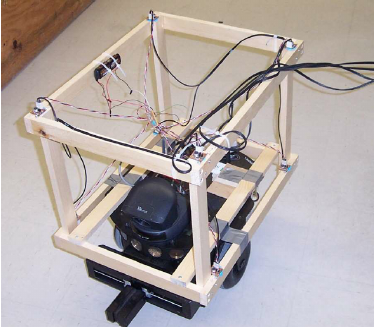
\includegraphics[width=0.75\textwidth]{./valin_2003/robot.png}
\centering
\caption{The microphone array on top of the mobile robot in \cite{valin_robust_2003}}
\label{fig:valin_2003_robot}
\centering
\end{figure}

\begin{figure}[H]
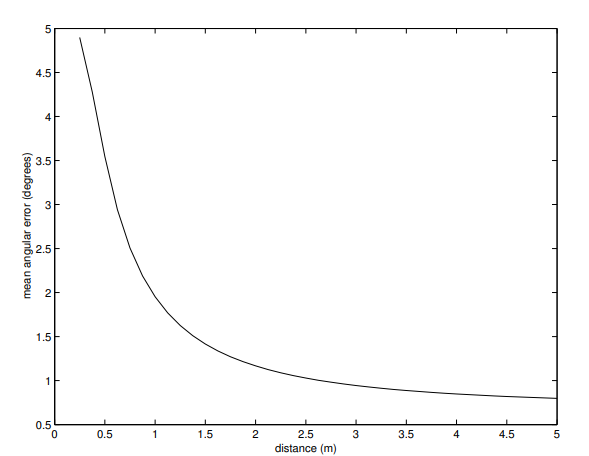
\includegraphics[width=0.75\textwidth]{./valin_2003/plot.png}
\centering
\caption{The mean angular error as a function of the distance between the source and the array in \cite{valin_robust_2003}}
\label{fig:valin_2003_plot}
\centering
\end{figure}

A similar approach \cite{hu_estimation_2009} proposed a novel estimation of the TDOA, namely eigenstructure-based GCC (ES-GCC) which can handle an unknown number of multiple sources. This paper could compute as before the three-dimensional bearing but also the distance for the near-field case, i.e. when the source is near enough to the array. The K-means++ algorithm was used to cluster accumulated results. This approach was tested on an array of eight microphones forming a rhomboidal prism seen in Figure-\ref{fig:hu_2009_plot}; the diagonal distances from the centre were 0.22 and 0.14 \si{m}. This was done in a real room for both a single source and multiple ones that were all 2.4 \si{m} away from the array. The worst SNR was 14.58 \si{dB}. The mean error for all experiments was less than 3 \si{\deg}. The estimation of distance was not evaluated, only the azimuth and elevation. The computation was not discussed nor was reverberation.
% multiple sources?

\begin{figure}[H]
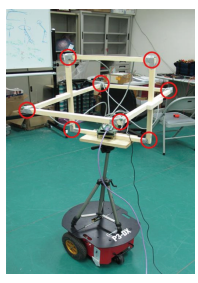
\includegraphics[width=0.75\textwidth]{./hu_2009/array.png}
\centering
\caption{The microphone array in \cite{hu_estimation_2009}}
\label{fig:hu_2009_plot}
\centering
\end{figure}

However, the former methods only compute the bearing, at least for the far field which is more relevant for the case with a smaller array. Another example \cite{chen_sound_2019} estimates the full three-dimensional coordinates of the source by an iterative algorithm based on Newton's method to solve a set of spatial coordinate relations. This example also had a few improvements such as a partitioning process, a fast search-strategy of the GCC peak, a screening strategy, and a new weighting function in the GCC that dealt with reverberation. However, this proposed weighting function needed beforehand the parameters of the environment and the rough displacement of the source; the authors have admitted that this limits the universality. In simulations, the improved weighting function gave a better distinct peak in the GCC for a reverberation-time of 300 \si{ms}. This method was tried on an array of five microphones forming a rectangular pyramid 0.25 \si{m} wide and 0.125 \si{m} tall as seen in Figure-\ref{fig:chen_2019_array}. The performance was tested at different points around the array from 1 to 6 \si{m} and with a SNR of 45 \si{dB}. The error in distance increased as the source was further away; this was observed at best as 0.05 \si{m} and at worst as 0.25 \si{m}. The error in azimuth varied little in both distance and bearing and was observed as being within 1.5 \si{\deg}. The performance was also tested at different levels of SNR, from 40 to 10 \si{dB}. In the worst case of 10 \si{dB}, the error in distance was observed at worst as 0.4 \si{m} seen in Figure-\ref{fig:chen_2019_distance_SNR}. The paper neglected any evaluation of the estimated elevation, considering that the geometry of the array is not symmetrical. Furthermore, the computational needs were not discussed in depth.

\begin{figure}[H]
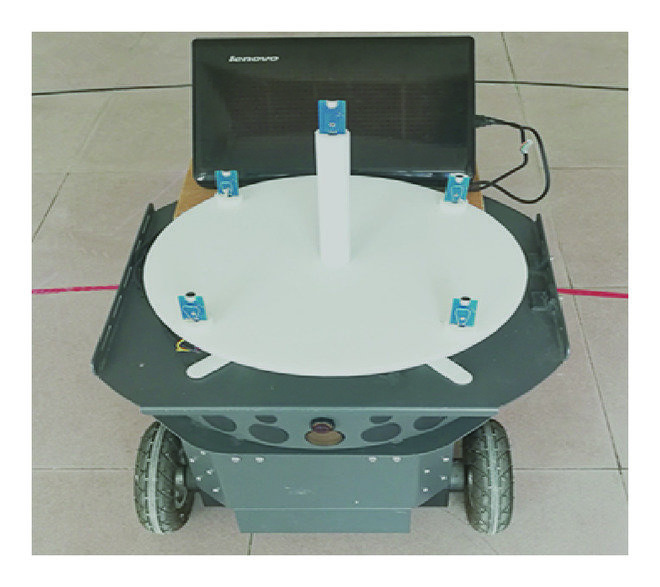
\includegraphics[width=0.75\textwidth]{./chen_2019/array.jpg}
\centering
\caption{The microphone array in \cite{chen_sound_2019}}
\label{fig:chen_2019_array}
\centering
\end{figure}

\begin{figure}[H]
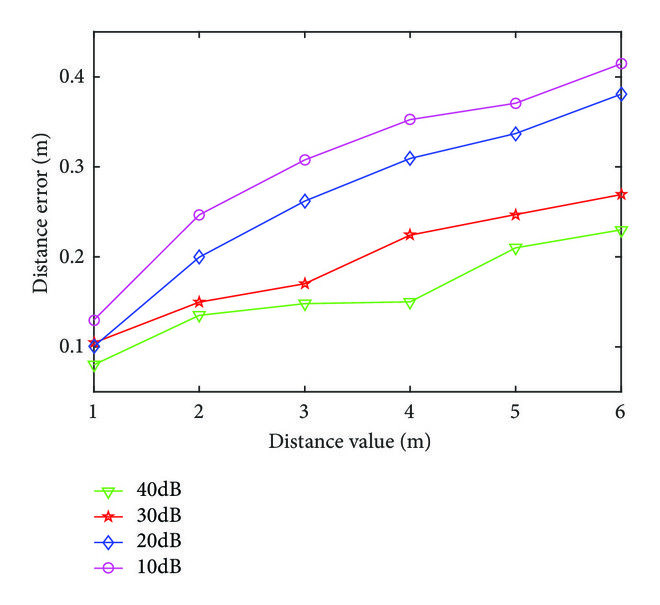
\includegraphics[width=0.75\textwidth]{./chen_2019/distance_SNR.jpg}
\centering
\caption{The error in distance as a function of distance for different SNRs in \cite{chen_sound_2019}}
\label{fig:chen_2019_distance_SNR}
\centering
\end{figure}

A similar paper \cite{bechler_system_2004} solved a similar set of equations but using Lagrange multipliers instead. It also applied tracking filtering such as an EKF. This approach was tested on an array of five microphones forming a double equilateral tetrahedron with sides 28 \si{cm} long. The SNR of the room was 15 \si{db}, and the room's reverberation-time at 60 \si{dB} was measured as 0.36 \si{s}. A number of sessions were tried where a speaking person moved along a different path. The mean squared error of the raw estimated position before filtering was observed to be at best 4.957 \si{\e{-3}}{$m^2$} and at worst 27.21 \si{\e{-3}}{$m^2$}. However, all the sessions had the speaker within 1 \si{m} of the array; so, they may be thought of as in the near field. Also, the paper makes no evaluation of the computation.

Likewise, another paper \cite{kim_robust_2008} employed robust spatial filtering, namely a Kalman filter, but only to estimate the azimuth. It used GCC-PHAT to estimate the TDOA but also used a trained feed-forward network of a single hidden layer to quantify the reliability of the estimated TDOA. 

Potential unwanted noise from servo-motors, etc., may affect and disrupt how well the system localises wanted sources. A very recent study \cite{manamperi_drone_2022} set out an approach that estimated the azimuth and elevation and mitigated the noise from a drone's motors. Here, the authors computed the GCC-PHAT as an angular spectrum for many pairs of microphones and summed each pair's angular spectra; this method is similar to SRP-PHAT in that the azimuth and the elevation corresponding to the largest sum belong to the estimated direction. In order to mitigate the motors' noise, the authors subtracted the known angular spectrum of the drone's motors from the mixed angular spectrum before summing. This known angular spectrum was computed from noise-only recordings with specific parameters of motor's current and speed. The tested drone had fifteen pairs of microphones seen in \ref{fig:manamperi_2022_array} and was tested in a semi-anechoic chamber with a reverberation-time of 20 \si{ms} at 20 \si{dB}. The drone was held resting at a height of 1 \si{m} above a circle of twelve sound-sources with a radius of 0.6 \si{m}. As seen in Figure-\ref{fig:manamperi_2022_map_n30}, the results showed acceptable accuracy of the proposed method compared to that of GCC-PHAT and of MUSIC for a SNR of at least -30 \si{dB}. The experiments were performed for multiple scenarios such as for a single source and for multiple.
% May be better in beamforming?

\begin{figure}[H]
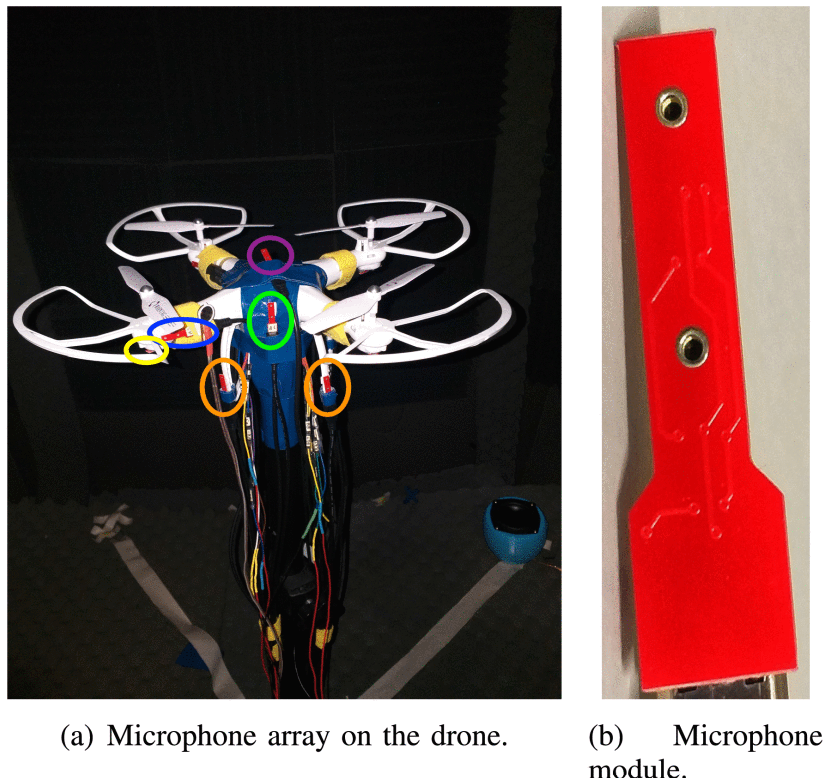
\includegraphics[width=0.75\textwidth]{./manamperi_2022/array.png}
\centering
\caption{The microphone array on the drone (a) and each pair (b) in \cite{manamperi_drone_2022}}
\label{fig:manamperi_2022_array}
\centering
\end{figure}

\begin{figure}[H]
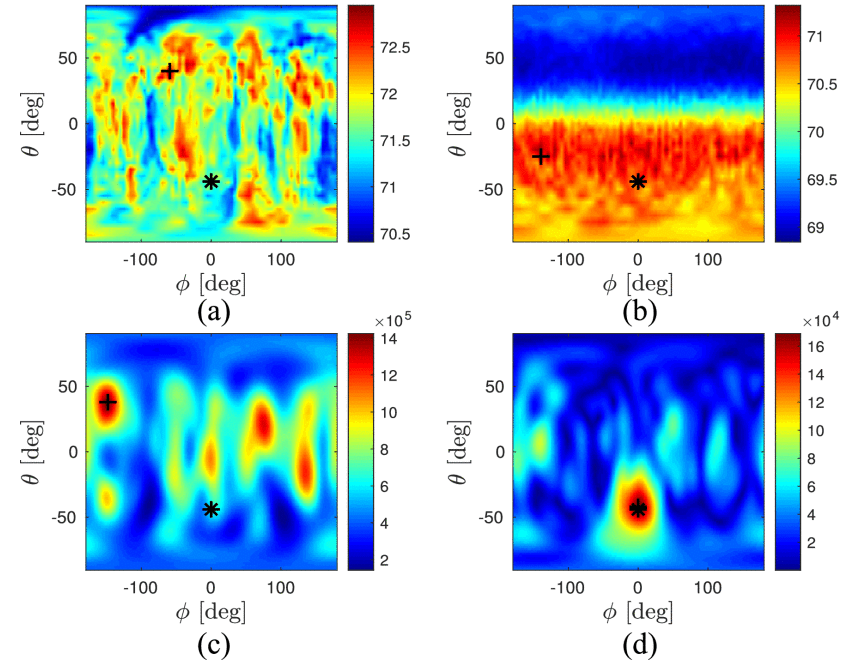
\includegraphics[width=0.75\textwidth]{./manamperi_2022/map_n30.png}
\centering
\caption{The energy maps for MUSIC (a), GEVD-MUSIC (b), GCC-PHAT (c), and the proposed method (d) at an SNR of -30 \si{dB} in \cite{manamperi_drone_2022}}
\label{fig:manamperi_2022_map_n30}
\centering
\end{figure}

Both two-dimensional and three-dimensional localisation was proposed in a paper \cite{mahajan_3d_2001} where a similar set of equations was solved, and the speed of sound could be estimated as a variable with at least six microphones. Where it was assumed to be constant, at least five microphones were needed instead. Only the two-dimensional case was evaluated in the preliminary testing. In which, the relative error in distance stayed below 1\%, and the worst error was 7.6 \si{mm} at 1 \si{m}, but this experiment was only done in a workspace $1000\times 1000$ \si{mm} and was done with ultrasonic pulses of 75 \si{kHz}. The authors did not reveal the geometry of the array and given how short the tested distances were, it may be assumed that the experiment was in the near field.

\subsubsection{Distance}

The estimation of distance is not very common in TDOA-based methods. Most examples only localise the direction, whether it is two-dimensional or three-dimensional. As said before, the TDOA yields a hyperbola or hyperboloid as the locus of the source. Therefore, a naive method would be to find the intersection given at least two pairs of microphones. However, error and noise of course make this hard as well as the computation in a robotics context.

Another way is to use two or more sub-arrays that yield single DOAs and are used to triangulate on a position \cite{rascon_localization_2017}. However, such a method would need sub-arrays that are far apart enough which is hard for a small robot where space is a luxury.

% The review has a few examples?

\subsubsection{Reverberation}

Reverberation is a big influence on the estimation of TDOA, especially in a room, since it leads to delayed reflections of the signal which show up in the GCC-PHAT. A statistical analysis \cite{gustafsson_source_2003} showed that the PHAT is the best estimator for the TDOA. The numerical examples in the paper showed good results as long as the reverberation-time was more than 0.07 \si{s}, the displacement between the microphones is longer than 0.2 \si{m}, and the distance between the source and the microphones is longer than 1.5 to 2 \si{m}. The same examples also showed that the probability of outliers was "tolerable" for a SRR more than 0 \si{dB}.

Another analysis \cite{brandstein_robust_1997} simulated three methods of estimating the TDOA, namely GCC-PHAT, GCC-ML, and Biweight. For all three, both the percentage of anomalies and the RMS error worsened for a reverberation-time longer than 0.1 \si{s}.

However, although GCC-PHAT generally handles reverberation well, it does not handle noise well across the spectrum since the algorithm gives all frequencies equal weight \cite{valin_robust_2003}. It especially does not do well with narrowband signals such as tones or voice.

\subsubsection{Multiple Sources}

Although the localisation of multiple sources has been explored for other methods such as beam-forming, it has not been explored much in TDOA-based methods. This is since most examples in the literature have been built on top of the basic idea of a single peak in the GCC-PHAT. However, the relationship between secondary peaks in the cross-correlation and other sources has been discussed.

Only a few basic studies in the fundamental relationship were done. A convention paper \cite{clifford_calculating_2010} proposed a method in the context of audio-engineering where multiple sources manifested themselves as distinct peaks in the GCC-PHAT. The results showed an accuracy of at least 85 \% where the SNR is at least 46.5 \si{dB}. However, the paper only considered the estimation of the TDOA in the context of musical instruments, not localisation, and the experiment was performed with little reverberation in mind. Another analysis \cite{kwon_analysis_2010} derived the mathematical cross-correlation function based on GCC-PHAT for multiple sources but did not seem to give much experimental data. 

Even so, no literature examples were found that exploited this relationship of secondary peaks for localisation in robotics \cite{rascon_localization_2017}. However, some studies have lately developed algorithms albeit not in a robotics context. A paper \cite{brutti_multiple_2010} proposed a method where an acoustic map, such as GCF or SRP-PHAT, is used to find the most dominant source which is then de-emphasised by lessening the GCC-PHAT at the time-delay corresponding to that source; this is repeated for the next most dominant source until all other located. However, the paper only tested this method for the near field.

Another paper \cite{boora_tdoa-based_2020} proposed a method of a delay density map made up of cubic subvolumes each of which weighted by a likelihood that a source is in it. The tested system had a resolution of 0.2 \si{m} and an RMS error at worst of about 0.6 \si{m} at an SNR of 5 \si{dB}. The experiments were tested for both the near field and the far field as well as for different arrays. The reverberation-times at 60 \si{dB} in such experiments were tested from 0.11 to 0.55 \si{s}. It also compared its own method with that of GCF-D (GCF De-emphasised) where theirs performed better.

Even given a method that only locates a single source at a time, one other way to find multiple sources is to cluster multiple estimated DOAs over many time-windows. One paper \cite{rascon_lightweight_2015} does such by tracking sources with a threshold on angle and smoothing such tracking with a Kalman filter. An adaptive variation of the K-mean++ algorithm has also been used to cluster multiple sources in an aforesaid paper \cite{hu_estimation_2009}.

\subsection{Beam-forming}

Beam-forming is a common technique in signal-processing and in many applications for both sound and radio. It is a method of setting many sensors or transmitters in such an array that waves at particular angles and areas constructively interfere to form a beam focused either on a chosen spot or in a chosen direction. Traditionally, it has been used in telecommunications so that multiple radio antennae form a beam that selectively transmits only in one direction. Here, for sound-source-localisation, it is used to steer a beam or a focus in a chosen direction or on a chosen spot so that the energy only from that location is measured. If the beam is steered in enough directions, then an energy map as a function of direction, e.g. azimuth, is made.

The simplest kind of beamforming is delay-and-sum beamforming where the signal from each microphone is delayed such that the overall sum of all the delayed signals corresponds to a steered direction \cite{rascon_localization_2017}. This sum is maximum when it is steered towards the source. The delay-and-sum beamformer's output steered at the position $\vec{r}_0$ for $M$ microphones is given as:
\begin{equation}
y_{\vec{r}_0}[t] = \sum_{m=1}^M x_m[t-\tau(\vec{r}_0)] 
\end{equation}
where $x_n$ is the signal from the $m$-th microphone, and $\tau(\vec{r}_0)$ is the TDOA corresponding at the position $\vec{r}_0$ \cite{argentieri_survey_2015}. In the far field, this output can be simplified to a direction $\theta_0$ instead of a position:
\begin{equation}
y_{\theta_0}[t] = \sum_{m=1}^M x_m[t-\tau(\theta_0)] 
\end{equation}
This output can yield an energy-map as:
\begin{equation}
E_{\vec{r}_0} = \sum_{t=1}^T y_{\vec{r}_0}[t]^2
\end{equation}
or
\begin{equation}
E_{\theta_0} = \sum_{t=1}^T y_{\theta_0}[t]^2
\end{equation}

A more general kind of beamforming is filter-and-sum beamforming where the signal from each microphone is filtered by its own linear filter rather than delayed \cite{argentieri_survey_2015}. The beamformer's output is given as:
\begin{equation}
y_{\vec{r}_0}[t] = \sum_{m=1}^M w_m(\vec{r}_0)[t]x_m[t]
\end{equation} 
where $w_m(\vec{r}_0)[t]$ is the impulse-response of the $m$-th linear filter.

One advantage of beamforming over basic localisation through TDOA is that multiple sources can be easily located since the method spatially filters, i.e. it only receives signals from a particular direction or space \cite{rascon_localization_2017}. However, if two sources are near to each other enough, then the resolution of the energy-map may not distinguish the two.

However, there are few considerations \cite{argentieri_survey_2015}:
\begin{itemize}
	\item The more microphones there are, the fewer side lobes or beams there are which show up beside the main lobe or beam.
	\item The further apart the microphones are, the narrower the beam is; this is particularly a problem for robotics where the room on a robot for an array is small.
	\item The beam is wider at lower frequencies; this affects the resolution and precision for locating sources of lower frequencies.
	\item Copies of the main lobe appear for high frequencies; this is a form of spatial aliasing. A Shannon spatial sampling theorem is given as $d<c/(2f_{\text{max}})$ \cite{argentieri_survey_2015}.
\end{itemize}

% peak is affected by SIR.

% high computation

\subsubsection{Literature Examples}

A robotic implementation \cite{valin_localization_2004} was done where the beamformer's energy was calculated in the frequency-domain using the cross-correlation weighted similarly to the authors' work with estimating the TDOA \cite{valin_robust_2003}. The authors claim that the spectral whitening before computing the beamformer's energy helps narrow the peaks. Here, the authors also proposed a spherical search-grid of 2562 points seen in Figure-\ref{fig:valin_2007_grid} where the beamformer's energy of each is computed. This grid yields a resolution of about 2.5 \si{\deg}. The direction, i.e. both the azimuth and the elevation, of the loudest source is found when the beamformer's energy is maximum. Thereafter, the cross-correlation is zeroed for that loudest source, and the search is repeated for the next loudest source. This is done for a predicted number of sources. If there are fewer sources than the set number, then a source is falsely detected. To handle this, the authors employed probabilistic post-processing to temporally smooth the estimations. Furthermore, in their experiments, they applied two estimators working together, namely a short-term estimator for two sources and a medium-term one for four. The experiments were performed with with eight microphones in an open rectangular prism ($0.5\times 0.4\times 0.36$ \si{m}) on top of a mobile robot in "a noisy environment with moderate reverberation"; in fact, this is the same array and robot in the authors' former work \cite{valin_robust_2003} as seen before in Figure-\ref{fig:valin_2003_robot}. The computation was done on a desktop PC and used about 30\% of the CPU. Firstly, the detection-rate was tested against distance for three kinds of sounds, namely hands clapping, speech, and a burst of white noise 250 \si{ms} long. The system was able to detect these sounds reliably up to 5 \si{m}, but drops around 7 \si{m}. The authors claimed that narrowband signals such as tones and speech were detected worse, whilst those with a broader band, such as noise, could be detected much better at longer distances. Furthermore, the estimated azimuth was accurate for four moving speakers although struggled to detect seven. Similar accuracies for both the azimuth and the elevation were given when the robot was moving instead; the authors claim that this demonstrates the robustness against the noise of the motors. Lastly, the array was shown to still be able work when it was not completely open.

\begin{figure}[H]
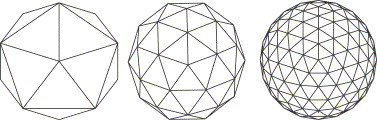
\includegraphics[width=0.75\textwidth]{./valin_2007/grid.jpg}
\centering
\caption{The evolution of the search-grid of 2562 points used in \cite{valin_robust_2003} and in \cite{valin_robust_2007}}
\label{fig:valin_2007_grid}
\centering
\end{figure}

The same authors later used the same beamforming method but with a particle filter instead \cite{valin_robust_2007}. It also involved a refined search after detecting a source that also estimated distance, but this estimated range was found to be too unreliable. It did however improve the accuracy of the direction in the near field. This new approach was tested on two different arrays on a different mobile robot seen in Figure-\ref{fig:valin_2007_array}. The first array, C1, was an open cube of eight microphones 15.5 \si{cm} wide, whilst the second, C2, was a closed square of four about 40 \si{cm} wide on the robot's chest. The experiments were tested in two different environments; the first environment, E1, was a medium-sized room with a reverberation time of 350 \si{ms} at - 60 \si{dB}, whilst the second, E2, was a hall with a reverberation-time of 1.0 \si{s}. In the first environment E1, the open array C1 detected sources more reliably than the closed array C2 within seven metres; C2 struggled to detect hand-claps specifically. Again, in E1, the RMS error for both the azimuth and the elevation was at worst 1.10 \si{\deg} for C1 and at worst 1.44 \si{\deg}. As before, experiments where either multiple sources were moving or the robot was moving were tested in both E1 and E2 as well as where the trajectories of two sources intersect. In such results, the system was deemed to track successfully as seen in Figure-\ref{fig:valin_2007_track}. Unlike the one before, this paper also discusses the computation needed, namely for the cross-correlation. For 1024 samples at 48 \si{kHz}, eight microphones, and 2562 searched directions, the complexity is claimed to be only 48.4 \si{Mflops} after counting all time-frequency transformations.

\begin{figure}[H]
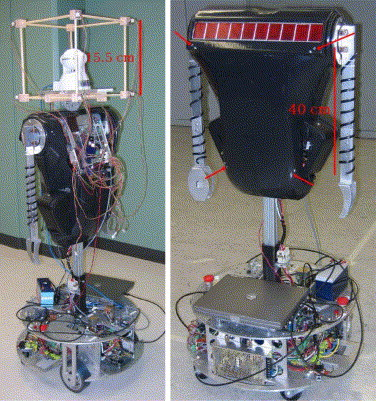
\includegraphics[width=0.75\textwidth]{./valin_2007/array.jpg}
\centering
\caption{The two different microphone arrays on the mobile robot, namely C1 on the left and C2 on the right, tested in \cite{valin_robust_2007}}
\label{fig:valin_2007_array}
\centering
\end{figure}

\begin{figure}[H]
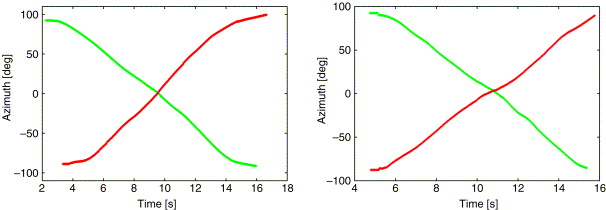
\includegraphics[width=0.75\textwidth]{./valin_2007/track.jpg}
\centering
\caption{The estimated azimuth of two tracked sources crossing paths tested in E1 on the left and in E2 on the right in \cite{valin_robust_2007}}
\label{fig:valin_2007_track}
\centering
\end{figure}

A further study \cite{badali_evaluating_2009} compared different variations and strategies of this kind of beamforming as well as the classic estimation of TDOA through GCC-PHAT. Here, TDOA-estimation from the peak of the GCC-PHAT (PEAK) was compared against a classic beamformer, called the steered-response-power (SRP) by the authors. Two variations were also considered, namely spectral weighting (SW) against SNR as proposed in \cite{valin_robust_2003}, \cite{valin_localization_2004}, \cite{valin_robust_2007} and direction-refinement (DR) as also studied in \cite{valin_robust_2007}. The latter is where a local search with a finer resolution is done after the initial search. Furthermore, two search grids are compared, namely a spherical rectangular grid (R) tessellated at 3600 points and a triangular element grid (T) of 2562 points. A cubical array of eight microphones with dimensions of 32 by 32 by 36 \si{cm} seen in Figure-\ref{fig:badali_2009_array} was tested. The experiments were done in a room with a reverberation-time of 0.1 \si{s}. The source playing pre-recorded sequences of speech was set at five points of different angle and distance as well as at two heights, one level with the robot and the other at the height of a human. The SNR received was varied by lowering the volume of the source. Two distinct experiments were done; in the first, only the background noise affected the accuracy which was observed to be Gaussian; in the second, a source of classical music as noise was set at only one of the tested positions. In the experiments, the mean error was measured against the SNR, and anomalies where the error was more than 10 \si{\deg} were counted as a percentage. From the results in Figure-\ref{fig:badali_2009_error_SNR}, the triangular grid was deemed better than the rectangular one given that the latter's resolution was not uniform and more concentrated at the poles of the sphere. Overall, the SRP with the SW performed worse than that without. The authors explained that this might have been the difficulty in estimating the noise spectrum. Furthermore, the SRP with the SW had more anomalies. The SRP was found to be better than the classic PEAK estimator.

\begin{figure}[H]
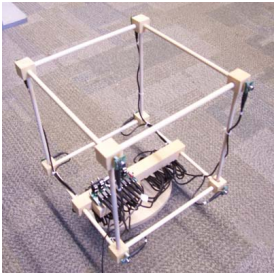
\includegraphics[width=0.75\textwidth]{./badali_2009/array.png}
\centering
\caption{The microphone array tested in \cite{badali_evaluating_2009}}
\label{fig:badali_2009_array}
\centering
\end{figure}

\begin{figure}[H]
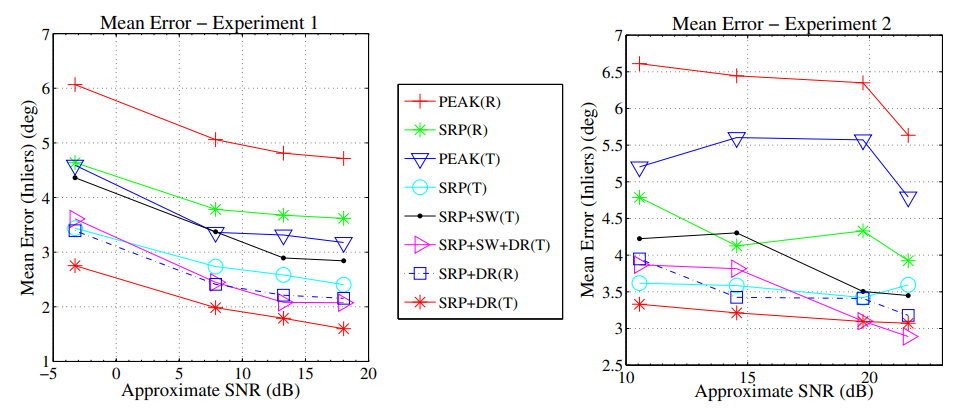
\includegraphics[width=0.75\textwidth]{./badali_2009/error_SNR.png}
\centering
\caption{The mean angular error as a function of SNR for different methods and configurations in \cite{badali_evaluating_2009}}
\label{fig:badali_2009_error_SNR}
\centering
\end{figure}

A more recent paper \cite{salvati_power_2019} proposed diagonal unloading on a beamformer so that the system could work with high noise. This diagonal unloading was done by subtracting a diagonal matrix from the covariance matrix of the array's signal. In the robust design, the covariance matrix was estimated by the largest eigenvalue of the array's signal which was computed by the power method. This robust design was evaluated in simulation and compared against the suboptimal design using diagonal unloading, SRP-PHAT, and MUSIC. The array was a uniform circle of eight microphones with a radius of 20 \si{cm}, and the spatial resolution was 5 \si{\deg}. As seen in Figure-\ref{fig:salvati_2019_RMSE_SNR}, when there was a single source, the RMS error in angle of the proposed design was at most about 2.5 \si{\deg} for an SNR of at least -10 \si{dB} and grew for worse SNR. As seen in Figure-\ref{fig:salvati_2019_RMSE_SNR_two}, when there were two sources, the RMS error was at most about 4 \si{\deg} for an SNR of at least -5 \si{dB}. In all cases, the proposed robust design worked better than SRP-PHAT and suboptimal design and did just as well as MUSIC. Furthermore, despite working just as well as MUSIC, the authors claimed that their proposed design has much simpler computation of $O(M^2)$ instead of that of $O(M^3)$ where $M$ is the number of microphones.

\begin{figure}[H]
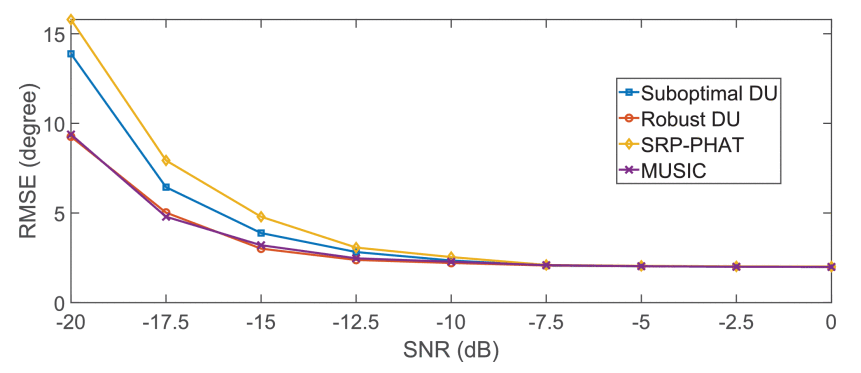
\includegraphics[width=0.75\textwidth]{./salvati_2019/RMSE_SNR.png}
\centering
\caption{The RMS error as a function of SNR for a single source in \cite{salvati_power_2019}}
\label{fig:salvati_2019_RMSE_SNR}
\centering
\end{figure}

\begin{figure}[H]
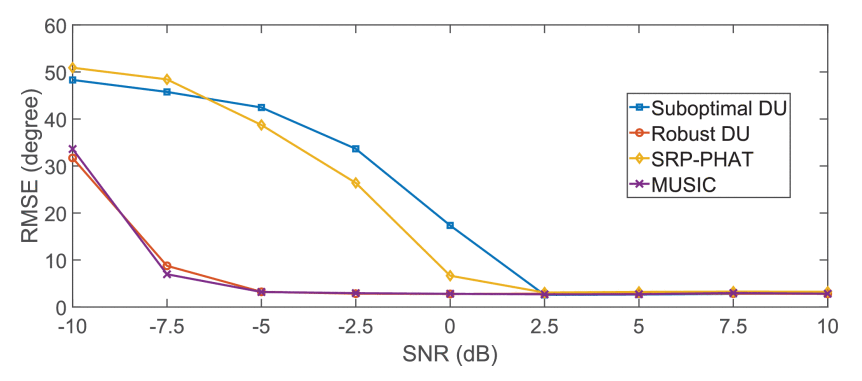
\includegraphics[width=0.75\textwidth]{./salvati_2019/RMSE_SNR_two.png}
\centering
\caption{The RMS error as a function of SNR for two sources in \cite{salvati_power_2019}}
\label{fig:salvati_2019_RMSE_SNR_two}
\centering
\end{figure}

The size of the array affects the beamformer. Firstly, the smaller it is, the wider the beam is especially for low frequencies. Secondly, the bigger it is, the more spatial aliasing there is, i.e. side lobes. Another recent study \cite{zhang_improved_2021} proposed a design to fix these two problems by employing an array UCCA of two concentric uniform circles of eight microphones for each. The first part of the design was frequency-classification-processing (FCP). Here, the signal's spectrum was split into bands, a lower and an upper one. A beamforming output was computed for each frequency bin. The smaller circle UCA1 used the upper band of frequencies, and the bigger circle UCA2 used the lower one. The two beamforming outputs were then summed together. The second part of the design is weighting each beamforming output; the best set of weights were found using particle-swarm-optimisation (PSO). The experimental array was made up a smaller circle of eight microphones with a radius of 10 \si{cm} and a bigger circle of eight with a radius of 20 \si{cm}. The experiment was done in an anechoic chamber and with two loudspeakers playing sounds of vehicle horns. Only the azimuth was tested. The proposed design worked better than the generic beamformer and had an error of 2 \si{deg} at worst as generally seen in the energy-maps in Figure-\ref{fig:zhang_2021_maps}.

\begin{figure}[H]
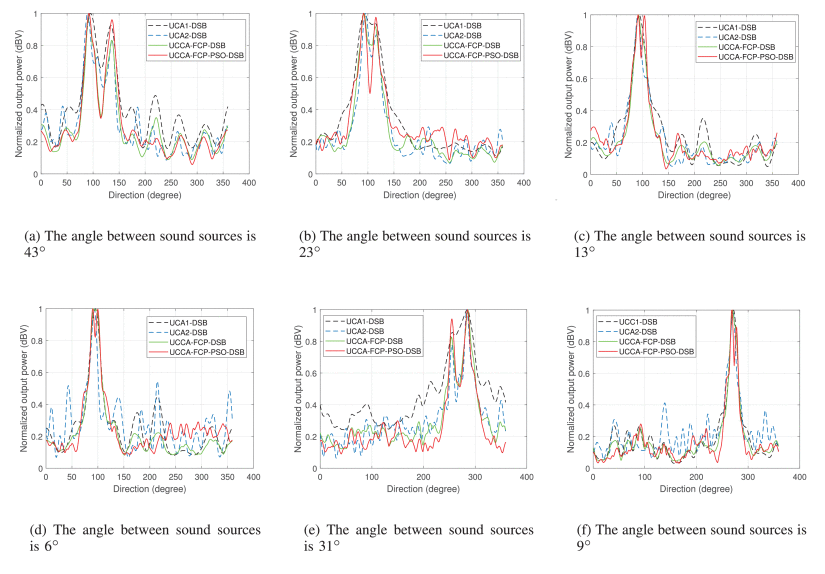
\includegraphics[width=0.75\textwidth]{./zhang_2021/maps.png}
\centering
\caption{The energy-maps of various delay-sum-beamformers (DSB) for two sources in \cite{zhang_improved_2021}}
\label{fig:zhang_2021_maps}
\centering
\end{figure}

Robotics is not the only application for localisation by beamforming. Autonomous drones are often imagined with the same capabilities of sound-source-localisation. One such study \cite{basiri_-board_2016} proposed SRP-PHAT but with a modified PHAT weighting with a power factor to mitigate the effect of noise. In order to localise multiple neighbouring drones, it also proposed a system inspired by \cite{brutti_multiple_2010} of pruning the next dominant source in the computed cross-correlation. The paper evaluated both a passive method of localising other drones' engine-sounds and an active method of localising other drones' beacons. The passive method which is the most relevant was tested indoors with a resting drone localising a flying drone. Motion-tracking was used to measure the true positions. The authors disclaimed that the sound of cooling fans belonging to eight tracking cameras and two computers could be heard in the room. For a single flying drone, the angular RMS error was 1.39 \si{\deg} as seen in Figure-\ref{fig:basiri_2016_histogram}. For multiple flying drones, the resting drone could localise at most three, and the precision worsen dramatically for the fourth. The array used for the passive method was a flat T-shape of four microphones seen in Figure-\ref{fig:basiri_2016_array}. The authors did not say what the exact dimension were. This study is of particular interest to robotics given that the system seemed to have been implemented on an embedded system on a drone, but the authors did not discuss computation, etc.

\begin{figure}[H]
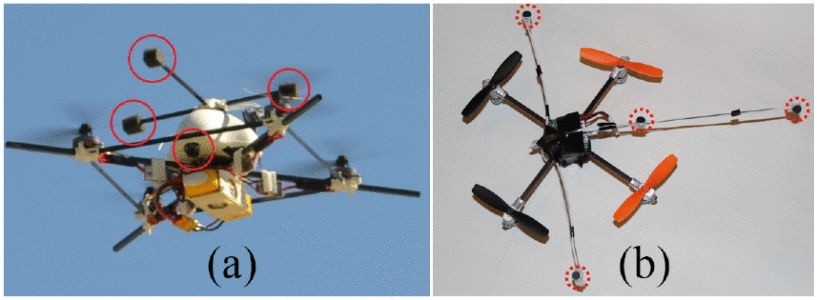
\includegraphics[width=0.75\textwidth]{./basiri_2016/array.png}
\centering
\caption{The two different microphone arrays tested in \cite{basiri_-board_2016}, namely one for the active method (a) and another for the passive method (b),}
\label{fig:basiri_2016_array}
\centering
\end{figure}

\begin{figure}[H]
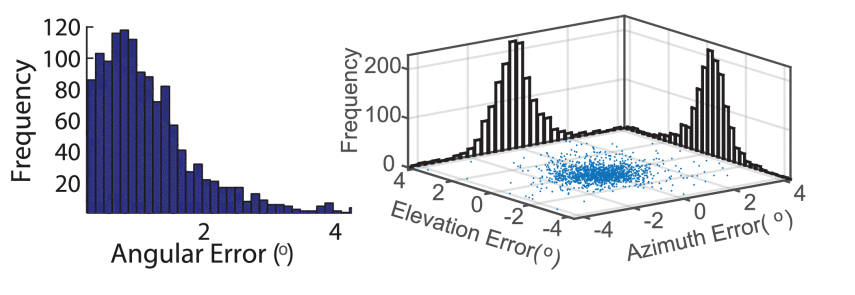
\includegraphics[width=0.75\textwidth]{./basiri_2016/histogram.png}
\centering
\caption{The histogram of the angular error for the passive method in \cite{basiri_-board_2016}}
\label{fig:basiri_2016_histogram}
\centering
\end{figure}

One paper \cite{tamai_three_2005} tested beamforming on two geometries, namely three rings of eight microphones and a larger ring of eight. The authors also proposed a method of separating sound-sources in frequency-domain, named frequency band selection (FBS), where two different directions of the beamformer are compared. However, this method works as long as the two sources do not overlap too much in the frequency-domain. Since the beam is wider at lower frequencies, a bandpass filter was applied between 1 and 3 \si{kHz}. In the experiments, the array of three rings was found to be more accurate than that of a single ring. The error in the azimuth of the first array was less than 3 \si{\deg} with one sound-source and less than 5 \si{\deg} with two, whilst the error in elevation was less than 6 \si{\deg} with one source. Also, the array of three rings was also able to estimate distance but only within one metre; the error of which was mostly within 300 \si{mm}.

A very basic implementation for tracking only the azimuth was tested on a mobile robot \cite{mattos_passive_2004}. Here, the robot was fitted with eight microphones around it and was able to track a sound-source reliably for frequencies tested from 200 \si{Hz} to 1.2 \si{kHz}.

\subsubsection{Frequency and Width}

As said before, the beam's shape is affected by the frequency of the received sound. Especially, the lower the frequency is the wider the beam is. This is a problem undergone in \cite{tamai_three_2005} where the band of observed frequencies has to be narrow, between 1 and 3 \si{kHz}. A frequency-invariant broadband beamformer using convex optimisation is proposed by a group for the far field \cite{argentieri_experimental_2005}, \cite{argentieri_prototyping_2005} and for the near field \cite{argentieri_modal_2006}.

\subsection{MUSIC}

One branch of methods used to analyse and locate sound-sources separates the space of signals into subspaces. The most common kind of which is multiple-signal-classification (MUSIC). This method has a very high resolution but generally has a high computational burden, especially compared to that of TDOA or beamforming. Therefore, it is not explored as in depth as before, but the general performance across the literature is given.

The basic idea behind MUSIC is that the signals received by an array of microphones is split into subspaces, each representing either a signal or a noise. The model for the signal received is:
\begin{equation}
X = W_s S + V
\end{equation}
where 
\begin{itemize}
	\item each row of $X\in \mathbb{C}^{M\times F}$ is the received signal of the $m$-th microphone $x_m$ in the frequency-domain, i.e. $X_m$,
	\item each row of $S\in \mathbb{C}^{N\times F}$ is the $n$-th source's signal $s_n$ in the frequency-domain, i.e. $S_n$,
	\item each row of $V\in \mathbb{C}^{M\times F}$ is the noise of the $m$-th microphones in the frequency-domain,
	\item $W_s\in \mathbb{C}^{M\times S}$ is a weighting that models the TDOAs of each source at each microphone for a given direction or position,
\end{itemize}
and where $M$ is the number of microphones, $F$ is the number of frequency-points, $N$ is the number of sources, i.e. signals \cite{rascon_localization_2017}. The weighting is written as:
\begin{equation}
W_s[f] = 
\begin{bmatrix}
	1 						& 1						& \cdots		& 1						\\
	e^{-2\pi f\tau_{2,1}}	& e^{-2\pi f\tau_{2,2}}	& \cdots		& e^{-2\pi f\tau_{2,N}}	\\
	e^{-2\pi f\tau_{3,1}}	& e^{-2\pi f\tau_{3,2}}	& \cdots		& e^{-2\pi f\tau_{3,N}}	\\
	\vdots					& \vdots					& \ddots		& \vdots					\\
	e^{-2\pi f\tau_{M,1}}	& e^{-2\pi f\tau_{M,2}}	& \cdots		& e^{-2\pi f\tau_{M,N}}
\end{bmatrix}
\end{equation}
where $\tau_{m,n}$ is the TDOA of the $n$-th source at the $m$-th microphone.

Given this, the overall goal of MUSIC is to split the space of signals into two subspaces, namely one for signals and another for noise. This is done by eigen-decomposition of the sampled covariance matrix $R[f]\in \mathbb{C}^{N\times N}$ for a given frequency $f$.

The most basic form of MUSIC, known as standard eigen-value-decomposition (SEVD), finds the eigen-decomposition of the covariance matrix as the following:
\begin{equation}
R[f] = Q[f]\Lambda[f]Q^{-1}[f]
\end{equation}
where $\Lambda[f]$ is a diagonal matrix of the $M$ eigenvalues $\lambda_m[f]$, and each column of $Q[f]$ is a corresponding eigenvector $q_m[f]$. This matrix of eigenvectors is often split into two subspaces, $Q[f] = [Q_s[f]|Q_n[f]]$, the former for signals, and the latter for noise \cite{rascon_localization_2017}. Thereby, the spatial spectrum is found from the orthogonality between the steered direction and the eigenvectors for noise:
\begin{equation}
P(\theta_0, \phi_0)[f] = \frac{\lvert A^*(\theta_0, \phi_0) A(\theta_0, \phi_0) \rvert}
	{\sum_{m=\tilde{N}+1}^M \lvert A^*(\theta_0, \phi_0) q_m[f] \rvert}
\end{equation}
where $\tilde{N}$ is the number of sources considered, and $A(\theta_0, \phi_0)\in \mathbb{C}^{M\times 1}$ is the steering vector of transfer-functions at each microphone for a given three-dimensional direction\footnote{Much like beamforming, a full three-dimensional position can more generally be considered rather than only a direction, but again like before, this only works reliably in the near field. Since the far field is much more relevant to a small array on a robot, only direction has been considered in this example.}, i.e. an azimuth $\theta_0$ and an elevation $\phi_0$ \cite{nakamura_real-time_2012}. More simply, each row is often the lag $e^{-2\pi f\tau_m}$ where $\tau_m$ is the TDOA at the $m$-th microphone corresponding to the given direction \cite{rascon_localization_2017}.

This spatial spectrum however is narrowband for one point or bin of frequency. For a broadband response, the narrowband response is averaged over the given band of frequencies \cite{ishi_effects_2011} \cite{nakamura_real-time_2012}.

An extension of SEVD is general eigen-value-decomposition (GEVD) where the noise is whitened before the decomposition \cite{nakamura_intelligent_2009} \cite{nakamura_intelligent_2011} \cite{nakamura_real-time_2012}. Here, the eigen-decomposition is such:
\begin{equation}
K^{-1}[f] R[f] = Q[f] \Lambda[f] Q^{-1}[f]
\end{equation}
where $K[f]$ is a freely chosen matrix but is often computed as $N[f]N^*[f]$ where $N[f]$ is the frequency-domain noise recorded when there are no signals. This is shown to be more robust than SEVD for a SNR less than 0 \si{dB}.

\subsubsection{Literature Examples}

One paper \cite{ishi_evaluation_2009} proposed a form of broadband SEVD-MUSIC where the output was the average of all the narrowband responses over a frequency-range. This was done for a small array of fourteen microphones around a robot's neck and chest as seen in Figure-\ref{fig:ishi_2009_array}. This proposed system estimated both the azimuth and the elevation on a discrete spherical grid with a resolution of about 5 \si{\deg}. Since MUSIC needs a known number of sources, the authors proposed a fixed number of sources for the narrowband MUSIC response and a maximum number of sources from the broadband response. They also compare the magnitude against a threshold to find whether the peak was a source or not. Multiple sources were nevertheless found by sequentially subtracting a two-dimensional Gaussian centred where the next highest source was; this approach is similar to others \cite{brutti_multiple_2010}, \cite{basiri_-board_2016}. The paper evaluated this system for a range of parameters, namely number of FFT points, frequency-range, and value of the threshold. The system was tested in a variety of "noisy environments", namely an office where the main sources of noise were an air-conditioner and the robot's hardware and an outdoor shopping mall, but the authors did not tell under what SNR and reverberation the system was tested. Nevertheless, the authors found that the system could run in real time given 64 FFT points for each frame which was about 4 \si{ms} long. Furthermore, the authors found that a frequency-range from 1 to 6 \si{kHz}, a threshold of 1.7, a fixed number of sources of 2, and a maximum number of sources of 5 were best. In most of the experiments, the accuracy was around 80 \% successful detection-rate.

\begin{figure}[H]
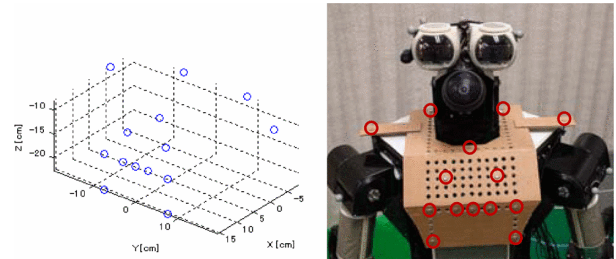
\includegraphics[width=0.75\textwidth]{./ishi_2009/array.png}
\centering
\caption{The microphone array on the robot tested in \cite{ishi_evaluation_2009}}
\label{fig:ishi_2009_array}
\centering
\end{figure}

Another kind of MUSIC is called GEVD-MUSIC which is more robust to noise, especially that more powerful than the wanted signal itself. An early paper \cite{nakamura_intelligent_2009} that first proposed this kind of MUSIC in the context of robotics compared the accuracy of GEVD-MUSIC as a percentage to that of SEVD-MUSIC. The accuracy of the latter dropped below an SNR of around 5 \si{dB} whilst the accuracy of GEVD-MUSIC kept at 100 \% at an SNR of around -7 \si{dB}. In a later paper \cite{nakamura_intelligent_2011}, many of the same authors proposed the same method but with a audio-visual integration with a particle filter for tracking inactive sources and hierarchical Gaussian mixture-models. Again, the accuracy of SEVD-MUSIC dropped at an SNR of around -8 \si{dB}, whilst that of GEVD-MUSIC dropped at an SNR of around -14 \si{dB}. 

To ease the computation, the same authors proposed a new kind of MUSIC called GSVD-MUSIC \cite{nakamura_real-time_2012}. To further lessen computation, the authors proposed a hierarchical search from coarse to fine, and to improve the resolution, they linearly interpolated the transfer-functions in both the frequency- and time-domain. The accuracy of the proposed GSVD-MUSIC only began to drop at an SNR fo around -10 \si{dB}, about 5 \si{dB} less than that of GEVD-MUSIC. The average error in the azimuth was at best about 1 \si{\deg} and at worst about 10 \si{\deg}. The proposed method also worked well for a moving source. The array was a circle of eight microphones embedded in the robot's head. The authors claimed that their new method of GSVD-MUSIC lessened the computational cost by 40.6 \% compared to GEVD-MUSIC and that their design of a hierarchical search lessened it by a further 59.2 \% for a single source. However, the computation was done on a laptop, and no comparison was made with other methods of sound-source-localisation such as SRP-PHAT.
% discussion: array on head

\begin{figure}[H]
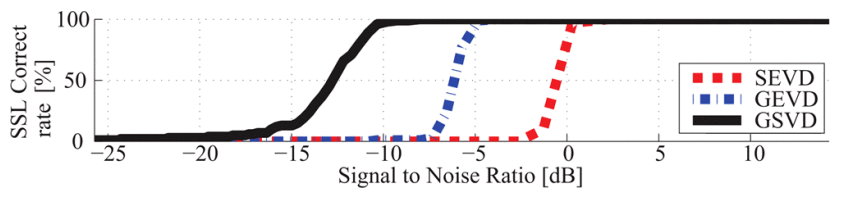
\includegraphics[width=0.75\textwidth]{./nakamura_2012/rate_SNR.png}
\centering
\caption{The rate of successful localisations against SNR for SEVD, GEVD, and the proposed GSVD in \cite{nakamura_real-time_2012}}
\label{fig:nakamura_2012_rate_SNR}
\centering
\end{figure}

\subsection{Discussion of Literature Examples}

Many examples and methods in the literature have been discussed. Here, a summary of the most relevant examples is given. The following attributes are compared:
\begin{itemize}
	\item the type of method, i.e. one of three categories discussed so far, namely TDOA, beamforming, and MUSIC,
	\item the specific method itself,
	\item the result or output of the algorithm, i.e. the type of localisation whether it is the direction only or the full three-dimensional coordinates (note that some methods could estimate distance but only in the near field; here, only the result in the far field is considered),
	\item the number of sources detectable, often either single or multiple,
	\item the accuracy or precision,
	\item the built-in resolution of the method,
	\item the number of microphones in the array,
	\item the array's dimensions (given a complex array, only the widest displacement is given),
	\item the distances tested,
	\item the noise under which the method was tested or for which it is rated, often given as the SNR,
	\item the reverberation under which the method was tested,
	\item the sampling rate,
	\item the length of the frame, window, or block of samples (may be in either number of samples or simply time),
	\item any comments on the computation, e.g. whether the method runs in real-time, what the method was computed on, etc.,
	\item and any comments about the design or method.
\end{itemize}

%\begin{landscape}
%
%\begin{tabular}{c | c c c c c c c c c c c c c c c}
%	\hline
%	Paper		
%		& Kind	
%		& Result
%		& Sources	
%			& Accuracy	
%			& Resolution
%				& Microphones	
%				& Dimensions	 
%					& Tested distances
%					& Noise
%					& Reverberation
%						& Sampling rate
%						& Frame-length
%						& Computation
%						& Context	
%						& Comments \\
%	\hline
%	\hline
%	Valin et al., 2003 \cite{valin_robust_2003}
%		& TDOA	
%		& 3D angle	
%		& single
%			& 0.6 - 4.9 \si{\deg} (MSE)
%			& ?
%				& 8		
%				& $0.5\times 0.4\times 0.36$ \si{m}
%					& 0.3 to 5 \si{m}
%					& "relatively high"
%					& "moderate"
%						& ?
%						& ?
%						& real-time, desktop computer, Athlon XP 2000+, 15 \% of CPU
%						& mobile robot
%						& Uses a modified weighting of GCC-PHAT dependent on SNR. Performs better for broadband signals \\
%	\hline
%	Hu et al., 2009 \cite{hu_estimation_2009}
%		& TDOA	
%		& 3D angle only in far field		
%		& multiple
%			& < 3 \si{\deg} (average error)
%			& ?
%				& 8
%				& rhombic prism 0.22 by 0.1 by 0.1 \si{m} 
%					& 2.4 \si{m}
%					& 14.58 \si{dB}
%					& ?, the room was $10.5 \times 7.2$ \si{m} and 3.6 \si{m} high
%						& 16 \si{kHz}
%						& ?
%						& ?
%						& mobile robot
%						& Uses adaptive K-means++ algorithm to track multiple sources. \\
%	\hline
%	Chen \& Xu, 2019 \cite{chen_sound_2019}
%		& TDOA
%		& full 3D coordinates
%		& single
%			& 0.4 \si{m}, 1.9 \si{\deg} \footnote{distance and azimuth respectively at worst at 6 \si{m} and 10 \si{dB}}
%			& ?
%				& 5
%				& rectangular pyramid 0.25 \si{m} wide 0.125 \si{m} tall
%					& 1 to 6 \si{m}
%					& 10 to 45 \si{dB}
%					& at most 300 \si{ms}
%						& ?
%						& ?
%						& real-time
%						& mobile robot
%						& Uses a variety of processing techniques such as a PHAT weighting robust to reverberation. \\
%	\hline
%	Bechler et al., 2004 \cite{bechler_system_2004}
%		& TDOA
%		& full 3D coordinates
%		& single
%			& 4.957 - 27.21 \si{\e{-3}}{$m^2$} (MSE)
%			& ?
%				& 5
%				& a double equilateral tetrahedron with sides 28 \si{cm} long
%					& within about 1 \si{m}
%					& 15 \si{dB}
%					& 0.36 \si{s} ($R_{60}$)
%						& 16 \si{kHz}
%						& 32 \si{ms}
%						& real-time
%						& robot audition
%						& Uses EKF to track sources. \\
%	\hline
%	Manamperi et al., 2022 \cite{manamperi_drone_2022}
%		& TDOA
%		& 3D angle
%		& multiple
%			& 0.05 - 9.43 \si{\deg}
%			& ?
%				& 30
%				& ?
%					& about 1.2 \si{m}
%					& from -15 to -30 \si{dB}
%					& 20 \si{ms} (at 20 \si{dB})
%						& 48 \si{kHz}
%						& 4096 samples
%						& real-time
%						& drone-audition
%						& Subtracts noise from the motors by formerly recorded data. \\
%	\hline
%	Valin et al., 2004 \cite{valin_localization_2004}
%		& Beamforming
%		& 3D angle
%		& multiple
%			& 100 - 42 \% (success-rate) \footnote{The latter is at worst for speech at 7 \si{m}.} 
%			& 2.5 \si{\deg}
%				& 8
%				& $0.5\times 0.4\times 0.36$ \si{m}
%					& from 3 to 7 \si{m}
%					& "noisy"
%					& "moderate"
%						& 48 \si{kHz}
%						& 1024 samples (with 50 \% overlap)
%						& real-time, desktop computer, Athlon XP 2000+, 30 \% of CPU
%						& mobile robot
%						& Uses probabilistic post-processing. \\
%	\hline
%	Valin et al., 2007 \cite{valin_robust_2007}
%		& Beamforming
%		& 3D angle
%		& multiple
%			& 1.10 \si{\deg}, 0.89 \si{\deg} (RMSE) \footnote{azimuth and elevation respectively}
%			& 2.5 \si{\deg}
%				& 8
%				& cube 15.5 \si{cm} wide
%					& from 1 to 7 \si{m}
%					& ?
%					& 350 \si{ms} ($R_{60}$)
%						& 48 \si{kHz}
%						& 1024 samples (with 50 \% overlap)
%						& real-time, 48.4 \si{Mflops}, 1.6 \si{GHz} Pentium-M CPU, 30 \% of CPU
%						& mobile robot
%						& Uses a particle-filter to track multiple sources. \\
%	\hline
%	Salvati et al., 2019 \cite{salvati_power_2019}
%		& Beamforming
%		& 3D angle
%		& multiple
%			& 2.5 \si{\deg} (RMS) \footnote{at worst for a single source at -10 \si{dB}}
%			& 5 \si{\deg}
%				& 8
%				& circle 40 \si{cm} wide
%					& ?
%					& 0 to 20 \si{dB} for a single source
%					& ?
%						& 48 \si{kHz}
%						& 2048 samples
%						& ? 
%						& drone
%						& Uses diagonal unloading to mitigate noise. \\
%	\hline
%	Zhang et al., 2021 \cite{zhang_improved_2021}
%		& Beamforming
%		& 3D angle
%		& multiple
%			& 2 \si{\deg} at worst
%			& ?
%				& 16
%				& two concentric circles, 20 and 40 \si{cm} wide
%					& about 1 \si{m}
%					& ?
%					& ?
%						& 204.8 \si{kHz}
%						& 5 \si{s}
%						& ?
%						& general
%						& Uses particle-swarm-optimisation. \\
%	\hline
%	Basiri et al., 2016 \cite{basiri_-board_2016}
%		& Beamforming
%		& 3D angle
%		& multiple
%			& 1.39 \si{\deg} (RMSE) \footnote{for a single source}
%			& ?
%				& 4
%				& T-shape
%					& ?
%					& ?
%					& ?
%						& 40 \si{kHz}
%						& 1024 samples
%						& Atmel AVR32 microcontroller
%						& drone-audition
%						& Proposed a modified PHAT to handle noise. \\
%	\hline
%	Ishi et al., 2009 \cite{ishi_evaluation_2009}
%		& MUSIC
%		& 3D angle
%		& multiple
%			& ~80 \% (success-rate)
%			& 5 \si{\deg}
%				& 14
%				& 40 \si{cm} wide overall
%					& ?
%					& ?
%					& ?
%						& 16 \si{kHz}
%						& from 64 to 512 samples
%						& real-time for at most 128 samples
%						& robot-audition
%						& Uses a fixed number of expected sources. \\
%	\hline
%	Nakamura et al., 2012 \cite{nakamura_real-time_2012}
%		& MUSIC
%		& 3D angle
%		& multiple
%			& 1 - 10 \si{\deg}
%			& 1 \si{\deg}
%				& 8
%				& circle
%					& 1 \si{m}
%					& ?
%					& 0.2 \si{s}
%						& 16 \si{kHz}
%						& 512 samples
%						& real-time, 2.0 \si{GHz} Intel Core i7 CPU
%						& robot-audition
%						& Uses a hierarchical coarse-fine search to reduce computation. \\
%	\hline
%\end{tabular}
%
%\end{landscape}

Nearly all methods only compute the three-dimensional angle. Only two attempt full three-dimensional position, i.e. direction along with distance. However, only Chen \& Xu in 2019 \cite{chen_sound_2019} seemed to attempt this in the far field for distances more than 1 \si{m}; Bechler et al. in 2004 \cite{bechler_system_2004} only have tested within about 1 \si{m} which may considered to be the near field given the dimensions of their array.

A common theme throughout the literature-review is the inconsistent calculation of accuracy. Some papers used the RMS error (RMSE), the mean-squared error (MSE), or simply the average error itself. Some papers did not even give error but rather the percentage of successful localisation relative to the resolution. Furthermore, it is hard to summarise the accuracy of a method given that it varies depending on noise, distance, etc. Here, the accuracy at best and at worst is given as lower and upper bounds. Nonetheless, most methods tended to have an error of 2 \si{\deg}.

Although some dimensions were not given at all, e.g. Basiri et al. in 2016 \cite{basiri_-board_2016}, the smallest array seemed to be that of Hu et al. in 2009 \cite{hu_estimation_2009}. The biggest was that of Valin et al. in 2003 and 2004 (both papers use the same array but different methods) \cite{valin_robust_2003} \cite{valin_localization_2004}.

As for noise, Manamperi et al. in 2022 \cite{manamperi_drone_2022} tested up to the worst SNR of -30 \si{dB} although this paper was specifically about mitigating noise in the context of drones. Whilst for reverberation, Bechler et al. in 2004 \cite{bechler_system_2004} had the longest reverberation-time of 0.36 \si{ms} at 60 \si{dB}. Again however, many papers neglect any information about noise or reverberation, some albeit with vague descriptions.

Most methods could run in real-time albeit on laptop and desktop computers. However, Basiri et al. in 2016 \cite{basiri_-board_2016} seemed to be the only example implemented on an embedded system on the drone itself, namely an Atmel AVR32 microcontroller. This example is therefore of particular interest to this project given the want for an embedded implementation.

% closed array

% noise-mitigation

\chapter{Simulation}

%\nocite{*}

\bibliographystyle{plain}
\bibliography{./zotero}

%\begin{figure}[!h]
%\includegraphics[width=1\textwidth]{image.png}
%\centering
%\caption{Caption,}
%\label{fig:image}
%\centering
%\end{figure}

%\includepdf[pages=-,pagecommand={},angle=90,width=\textwidth]{controller_1.pdf}
%\includepdf[pages=-,pagecommand={},angle=90,width=\textwidth]{regulator_1.pdf}
%\includepdf[pages=-,pagecommand={},angle=90,width=\textwidth]{timer_1.pdf}


\end{document}
